{\sanhao\heiti\filcenter \centerline{本科毕业论文外文翻译}}
文献原文:\\
Kim Y, Jernite Y, Sontag D, et al. Character-aware neural language models[J]. arXiv preprint arXiv:1508.06615, 2015.\\
{\sihao\songti\filcenter \centerline{\textbf{以字为单位的自然语言模型}}}

\section*{摘要}
\addcontentsline{toc}{section}{摘要}
  我们描述了一个只依赖以字为单位输入的自然语言模型。我们的预测依然基于以词为单位。我们的模型对于字使用了
  卷积神经网络(CNN)和高速网络,模型的输出将作为输入,输入到由长短期记忆人工神经网络神经元(LSTM)组成的循环神经网络(RNN)。
  对于Penn Treebank英文数据集,我们的模型比现存的主流模型的参数少60\%,却仍然能取得不相上下多结果。对于内含丰富词法的语言(比如阿拉伯语、捷克语、法语、德语
  西班牙语、俄语),我们的模型的在需要很少的参数的情况下,表现超过LSTM的基准线。我们的结果表明,对于很多语言来说,以字为单位的输入,已经足够对语言建模。
  进一步分析由我们模型的产生的词的表示表明,我们的模型能够基于字编码并且包含语义信息。

\section{介绍}
语言建模是人工智能和自然语言处理最基础的任务。一个语言模型是对于一系列词的概率分布和转换方法。其中,转换方法通常包括通过计数和子序列拟合对马尔科夫链第n次序的假设和估测n-gram的概率。基于计数的模型比较容易训练,但是对于稀有词,可能由于数据稀疏而不能很好的估计。
\\
神经语言模型为了解决n-gram数据稀疏问题通过参数把词向量化(词嵌入),并把向量词作为神经网络的输入。向量化所使用的参数在训练中学习到。
通过神经语言模型获得的词嵌入具有语义上比较接近的词在向量空间比较接近这一性质。\\
虽然神经语言模型的表现优于计数语言模型,但是该模型不能表示语素信息。比如,该模型不能发现相同前缀的词(例如eventfull,eventfully,uneventful,uneventfully)是结构上有关联的,他们应该在向量空间上结构相关。因此,稀有词的嵌入可能被错误的估计。这个问题对于词法丰富的语言来说,问题尤其严重\\
在这篇文章中,我们提出了一个语言模型,这个模型通过以字为单位的卷积神经网络来获取子词信息。模型的输出将作为RNN语言模型的输入。不同于之前使用词素来获取子词信息的模型,我们的模型不需要对词素标记。同样,不同于近期提出的结合词嵌入和字节的模型,我们的模型在输入层不使用词嵌入。因为对于神经语言模型,大多数的参数都是用于生产词嵌入,我们的模型
所需的参数相比于之前的模型显著减少。特别适用于对于模型大小有限制的平台。\\
作为总结,我们的贡献主要有下面几点:\\
\begin{itemize}
\item 对于英语,在Penn Treebank英文数据集上,我们的模型比现存的主流模型的参数少60\%,却仍然能取得不相上下多结果
\item 对于内含丰富词法的语言(比如阿拉伯语、捷克语、法语、德语、西班牙语、俄语),我们的模型的在需要很少的参数的情况下,表现超过LSTM的基准线
\end{itemize}
\section{模型}
Figure 1直观的显示了我们模型的架构。经典的神经语言模型采用词嵌入作为输入,我们的模型采用单层字节max-over-time池化卷积神经网络的输出作为输入\\
作为记号,我们用粗体小写字母标记向量,粗体大写字母标记矩阵,斜体小写字母标记变量,花体大写字母标记集合。为了标记方便,我们假设字和词都已经转换成了索引。\\
\begin{figure}[h]
  \centering
  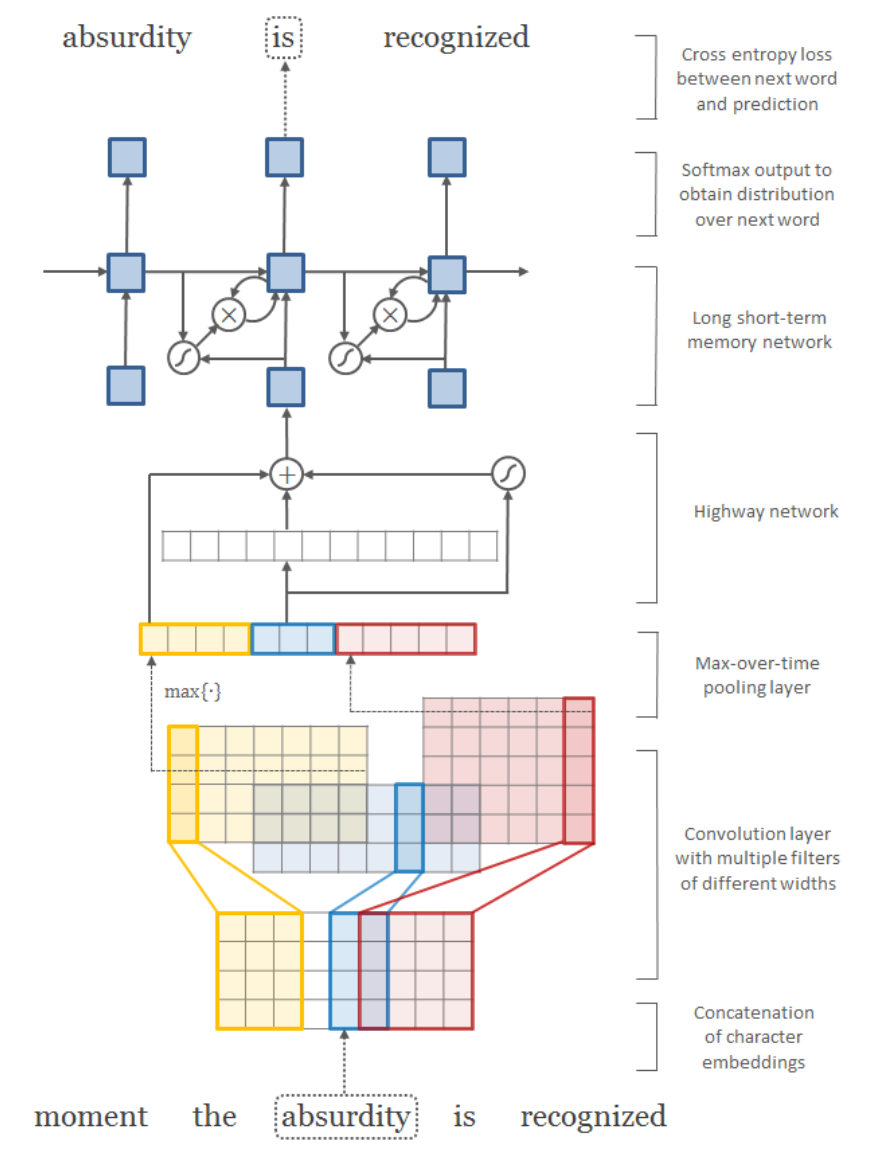
\includegraphics[width=0.6\textwidth]{./images/figure1}
  \caption{模型架构}
\end{figure}
\subsubsection{递归神经网络}
递归神经网络(RNN)特别适合对于时序模型建模。在每一个时步$t$,根据输入向量$\bf{x}_{i} \in \mathbb{R}^{n}$、隐式状态$\bf{h}_{i}$,应用下面的公式产生下一层隐式状态:\\
\begin{equation}
\bf{h}_{i} = f(\bf(Wx)_{i}+\bf{Uh}_{t-1}+\bf{b})
\end{equation}
在这里$\bf{W} \in \mathbb{R}^{m x n},\bf{U} \in \mathbb{R}^{m x n},\bf{b} \in \mathbb{R}_{m}$都是仿射变换的参数,$f$是非线性对每个元素的函数。理论上,RNN中的隐式状态$\bf{h}_{t}$包含了t个时步的历史信息。然而在实际中,由于权重指数级爆炸或消失的问题,基本的RNN难以捕捉长期时间关联。\\
长短期记忆(LSTM)通过将RNN在每一时步增加一个记忆单元向量$\bf{c}_{i} \in \mathbb{R}_{n}$来解决这一问题。具体来讲,LSTM的每一步利用输入$\bf{x}_{i},\bf{h}_{t-1},\bf{c}_{t-1}$根据下面的公式,计算出$\bf{h}_{t},\bf{c}_{t}$:\\
\begin{equation}
\bf{i}_{t} = \sigma(\bf{W}^{i}\bf{x}_{i}+\bf{U}^{i}\bf{h}_{t-1}+\bf{b}^{i})
\end{equation}
\begin{equation}
\bf{f}_{t} = \sigma(\bf{W}^{f}\bf{x}_{t}+\bf{U}^{f}\bf{h}_{t-1}+\bf{b}^{f})
\end{equation}
\begin{equation}
\bf{o}_{i} = \sigma(\bf{W}^{o}\bf{x}_{t}+\bf{U}^{o}\bf{h}_{t-1}+\bf{b}_{o})
\end{equation}
\begin{equation}
\bf{g}_{t} = tanh(\bf{W}^{g}\bf{x}_{t}+\bf{U}^{g}\bf{h}_{t-1}+\bf{b}_{g})
\end{equation}
\begin{equation}
\bf{c}_{t} = \bf{f}_{t}\odot\bf{c}_{t-1}+\bf{i}_{t}\odot\bf{g}_{t}
\end{equation}
\begin{equation}
\bf{h}_t = \bf{o}_{t}\odot tanh(\bf{c}_{t})
\end{equation}
在这里$\sigma(\cdot)$和$tanh(\cdot)$是对每个元素的sigmoid函数和双曲正切函数,$\odot$是元素间相乘运算符,$\bf{i}_{t},\bf{f}_{t},\bf{o}_{t}$分别是输入门、遗忘门、输出门。当$t=1$时,$\bf{h}_{0}$和$\bf{c}_{0}$被初始化为零向量。LSTM需要的参数是$\bf{W}_{j},\bf{U}_{j},\bf{b}_{j},j\in\{i,f,o,g\}$\\
LSTM中的记忆单元是随时间变化的,从而缓解了权重指数消失问题。虽然权重指数爆炸仍然是一个问题,但是在实际训练过程中,一些简单的优化策略(例如变化率截断)效果很好。LSTM在包括语言建模在内的很多任务中显示出比基本RNN更好的结果。通过使$\bf{h}_{t}$作为$t$时的输入,可以很容易的将RNN/LSTM扩展到多层。实际上,在很多任务中,使用多层网络是获得有竞争力结果的关键选择\\
\subsection{Recurrent Neural Network Language Model}
记$\mathscr{V}$为固定的词汇集大小。给定历史序列$w_{1:t}=[w_{1},...,w_{t}]$,一个语言模型确定了$w_{t+1}$的概率分布。一个循环神经网络语言模型(RNN-LM)通过对隐式层应用仿射变换然后再应用softmax函数来实现这一点:\\
\begin{equation}
Pr(w_{t+1}=j\mid w_{1:t}) = \frac{exp(\bf{h}_{t}\cdot \bf{p}^{j}+q^{j})}{\sum_{j^{\prime} \in \mathscr{V}} exp(\bf{h}_{t}\cdot\bf{p}^{j^{\prime}}+q^{j^{\prime}})}
\end{equation}
在这里$\bf{p}^{j}$是$\bf{P} \in {\mathbb{R}}^{m \times |  \mathscr{V} |}$的第$j$列,$q^j$是偏差项。同样的,传统的RNN语言模型把词作为输入,如果$w_{t} = k$,传统模型在时步$t$的输入是$\bf{X} \in \mathbb{R}^{n \times | \mathscr{V} |}$的第$k$列$x^{k}$。
我们的模型把词嵌入矩阵$\bf{X}$替换成了下面描述的字为单位的卷积神经网络的输出。\\
我们记$w_{1:T}=[w_{1},...,w_{T}]$为训练词库的词序列,训练包括最小化该序列的负log概率(NLL),这一过程通常有啊截断反向传播来实现
\begin{equation}
NLL = - \sum_{t=1}^{T}logPr(w_t \mid w_{1:t-1})
\end{equation}
\subsubsection{字单位的卷积神经网络}
在我们的模型中,$t$时刻的输入是字单位的卷积神经网络的输出(CharCNN),我们将在这里小节里面描述CharCNN。CNN在计算机视觉领域的应用已经取得了突出的效果,并且对于多种自然语言处理(NLP)任务也是十分有效的。
针对NLP应用CNN有不同的架构,因为NLP需要时序卷积而不是空间卷积。\\
令$\mathscr{C}$为字的集合,$d$为字嵌入的维度,$\bf{Q} \in \mathbb{R}^{d \times | \mathscr{C} |}$为字嵌入矩阵。假设词$k \in \mathscr{V}$是由字序列$[c_1,...,c_l]$组成,$l$是词$k$的长度。
$k$的字表示由矩阵$\bf{C}^k \in \mathbb{R}^{d \times l}$给出,该矩阵的第$j$列是字$c_j$的字嵌入\\
我们对$\bf{C}^k$和宽度为$w$的过滤器$\bf{H} \in \mathbb{R}^{d \times w}$应用窄卷积。然后,我们加上偏差,再应用一个非线形函数来获得一个特征图谱$\bf{f}^k \in \mathbb{R}^{l - w + 1}$。$\bf{f}^k$的第$i$项由下式得出:\\
\begin{equation}
\bf{f}^k[i] = tanh(\langle \bf{C}^k[*,i:i+w-1],\bf{H}\rangle + b)
\end{equation}
在这里$bf{C}^k[*,i:i+w-1]$是$\bf{C}^k$的$i$到$i+w-1$列,$\langle \bf{A},\bf{B} = Tr(\bf{AB}^T)\rangle$是Frobenius内积。最后我们应用max-over-time作为过滤器$\bf{H}$对应的特征\\
\begin{equation}
y^k = max_i\bf{f}^k[i]
\end{equation}
这样做的目的是对于一个给定的过滤器,获取最重要的特征,也就是具有最高值的特征。一个过滤器本质上是选出一个字$n$元语法,$n$的大小由过滤器宽度决定。\\
我们通过一个特征由一个过滤矩阵得出描述了这个过程。我们的CharCNN使用多个不同宽度的过滤器获得$k$的特征向量。所以如果我们有$h$个过滤器 $\bf{H}_1,...\bf{H}_h$,就有$k$的输入表示$\bf{y}^k = [y^k_1,...,y^k_h]$,
对于很多NLP应用$h$通常在$[100,1000]$这个范围内选择。\\
\subsection{高速网络}
我们只需要在RNN-LM中在t时刻,用$\bf{y}^k$替换$\bf{x}^k$,正如我们稍后将要证明的,这样就已经能有很高效的表示了。我们也可以对$\bf{y}^k$使用一个多层感受器(MLP),来建模过滤器选择的n元语法的交集,但是我们发现这样的表现不是很好。\\
我们通过将$\bf{y}^k$运行在高速网络上进一步提高的我们的表现。高速网络是一层的MLP应用了仿射变换之后再施加一个非线形函数,从而得到一组新的特征。\\
\begin{equation}
\bf{z} = g(\bf{Wy} + \bf{b})
\end{equation}
一层高速网络实现了做了下面的过程:\\
\begin{equation}
\bf{z} = \bf{t} \odot g(\bf{W}_H\bf{y}+\bf{b}_H) + (\bf{1} - \bf{t})\odot \bf{y}
\end{equation}
在这里$g$是一个非线性函数,$\bf{t} = \sigma(\bf{W}_T\bf{y}+\bf{b}_T)$被称作转换门,$ (\bf{1} - \bf{t})$被称作进位门。
与LSTM网络中的记忆单元相似,高速网络会使一些维度的输入直接作为输出。在构建的时候,$\bf{y}$和$\bf{z}$的维度必须相同,$\bf{W}_T$和$\bf{W}_T$都是方阵。

\section{实验设置}
根据语言建模的标准,我们使用复杂度(PPL)来衡量我们模型的表现。对于一个序列$[w_1,...,w_T]$,一个模型的复杂度由下式给出:\\
\begin{equation}
  PPL = exp(\frac{NLL}{T})
\end{equation}
在这里NLL是对测试集来计算的。我们针对不同的语言和不同大小的词汇集进行了测试。\\
针对Penn Treebank(PTB)数据集,我们进行了高阶参数查询、模型检查和分离学习。使用0-20进行标准学习、21-22进行验证、23-24进行测试。PTB有一百万个标签,$| \mathscr{V} | = 10k$,已经被广泛的用于语言建模。\\
在针对PTB数据集优化高阶参数之后,我们将模型应用于很多词法丰富的语言:捷克语、德语、法语、西班牙语、俄语、阿拉伯语。尽管未经处理的数据是公开可用的,我们从作者那里获取到了预处理过的数据,他们的NLM充当了我们模型的基准。我们在每个语言有一百万个标签的小数据集(DATA-S)和$| \mathscr{V} | = 10k$远大于PTB的大数据集(DATA-L)上都进行了训练。\\
在这些数据集中,只有只出现一次的词汇会被<unk>替换,所以我们有效的使用了数据集上包含的词汇集。\\
\begin{figure}[h]
  \centering
  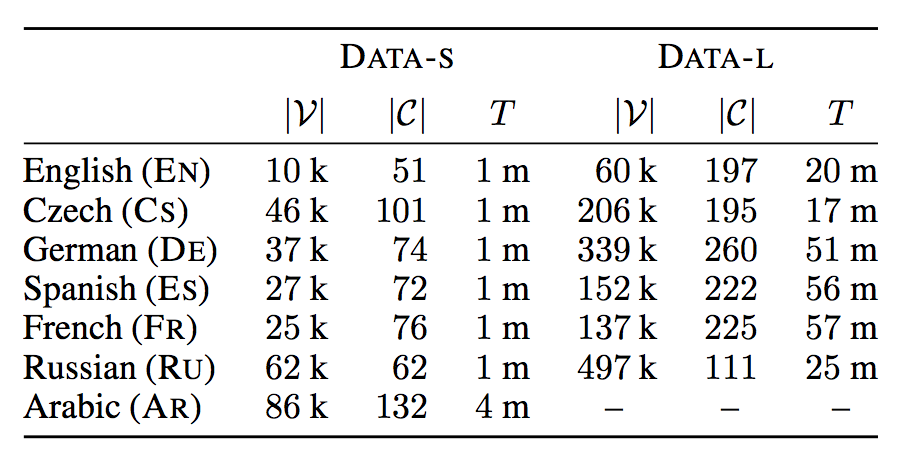
\includegraphics[width=0.6\textwidth]{./images/table1}
  \caption{词汇集统计数据}
\end{figure}


\subsection{优化}
我们使用截断反向传播来训练我们的模型。我们使用stochastic gradient descent反向传播35个时步。学习率初始设为1.0,当PPL没有在每个epoch在验证集下降超过1.0时,学习率变为原来的一半。\\
在DATA-S上,我们令batch大小为20,在DATA-L中我们使用batch大小为100。变化率是每个batch的平均。我们对于非阿拉伯语训练25个epoch,对于阿拉伯语训练30个epoch,选出在验证集上表现最好的模型。模型随机初始化为服从[-0.05,0.05]上的均匀分布。\\
我们在LSTM从输入到隐式层和softmax到输出层使用概率为0.5的丢弃法进行正规化学习。我们进一步限制变化率的范数小于5。如果$L_2$规范化的变化率超过5,在更新之前,我们设置他为5。变化率范数限制对于训练模型是很重要的。我们的选择很大程度上是受Zaremba et al.做的工作的启发。\\
最后,为了加速DATA-L上的学习,我们使用了hierarchical softmax。Hierarchical softmax是一个训练$| \mathscr{V} |$大小不同的语言模型的常用策略。我们选择$c = \lceil \sqrt{| \mathscr{V} |}  \rceil$个簇,随机的把$\mathscr{V}$分成大小相同的子集$\mathscr{V}_1,...,\mathscr{V}_c$,这样就有:\\
\begin{equation}
Pr(w_{t+1} = j \mid w_{1:t}) = \frac{exp(\bf{h}_t \cdot \bf{s}^r + t^r)}{\sum_{r^\prime = 1}{c} exp(\bf{h}_t \cdot \bf{s}^{r^\prime} + t^{r^\prime})} \times \frac{exp(\bf{h}_t \cdot \bf{p}^j_r + q^j_r)}{\sum_{j^\prime \in \mathscr{V}_r}exp(\bf{h}_t \cdot \bf{p}_r^{j^\prime} + q_r^{j^\prime})}
\end{equation}

在这里$r$是簇的索引,有$j \in \mathscr{V}_r$。上式的第一项是选择第$r$簇的概率,第二项是已知第$r$簇被选的情况下选中词$j$的概率。

\section{实验结果}
\subsection{English Penn Treebank}
\begin{figure}[h]
  \centering
  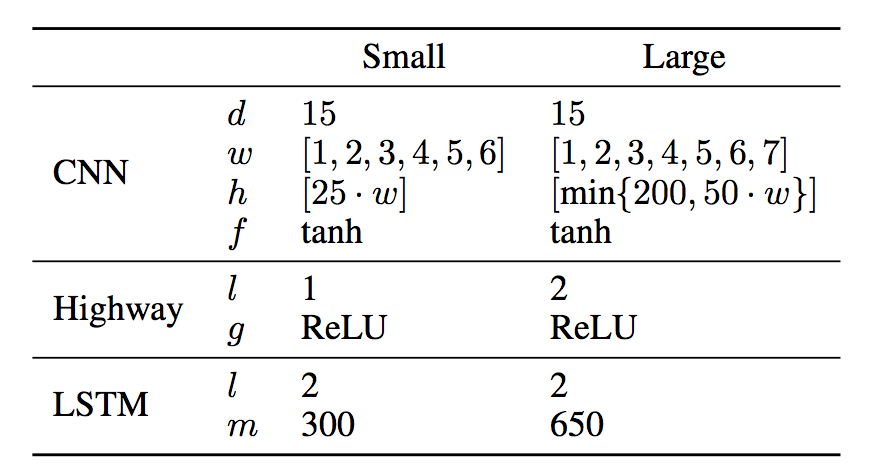
\includegraphics[width=0.6\textwidth]{./images/table2}
  \caption{小模型和大模型的架构}
\end{figure}
我们为了评估性能和大小的取舍,对我们的模型训练了两个版本。小模型(LSTM-Char-Small)和大模型(LSTM-Char-Large)的架构在表2中进行了总结。\\
和其他基准一样,我们也用词嵌入训练了两个比较模型(LSTM-Word-Small,LSTM-Word-Large)。LSTM-Word-Small使用了200个隐式单元。LSTM-Word-Large使用了650个隐式单元。词嵌入的大小分别是200和650.这些大小的选择是为了保持和字单位模型相似的参数数目。\\
正如从表3中看到的,我们的模型在参数少60\%的情况下,与现在领先的模型取得差不多的表现。我们的小模型明显优于其他大小相似的NLM。\\
\begin{figure}[h]
  \centering
  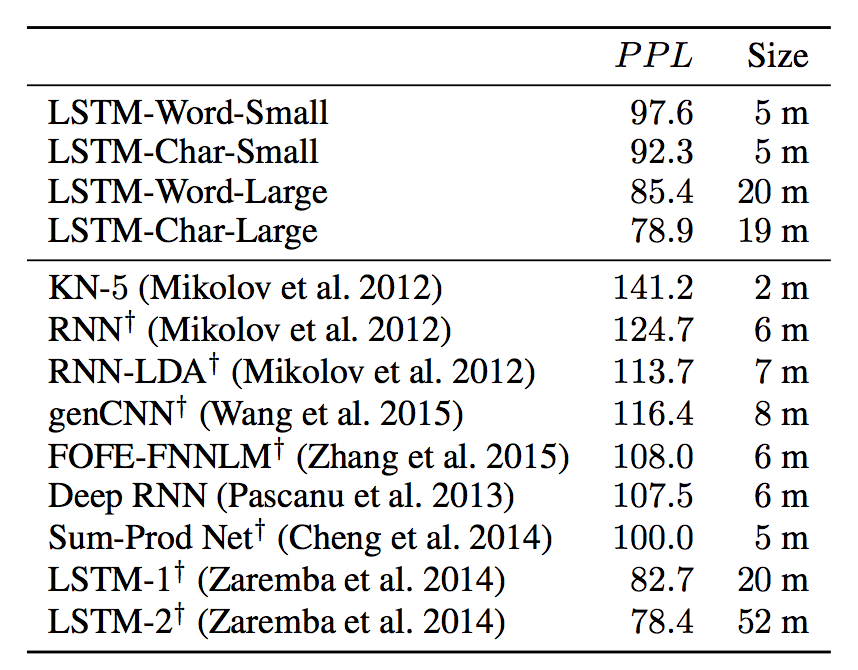
\includegraphics[width=0.6\textwidth]{./images/table3}
  \caption{小模型和大模型的架构}
\end{figure}

\subsection{其他语言}
我们模型在English PTB上的优异表现表明可以使用它来处理更大规模大数据。然而,英语从词法角度讲是相对简单的,所以我们下一部分的结果主要集中在有更丰富词法的语言上。\\
我们将我们的结果同morphological logbilinear (MLBL) 模型相比较。MLBL通过在输入和输出阶段的语素嵌入也考虑了子词信息。因为在同MLBL比较时,我们使用的LSTM比MLBL使用的feed-forward有众所周知的更优异的表现,我们又训练了一个LSTM版本的语素NLM。这个版本中,传入LSTM的词表示是词的语素嵌套的和。具体来讲,假设$\mathscr{M}$是一个语言的语素集,
$\bf{M} \in \mathbb{R}^{n \times | \mathscr{M} |}$是语素嵌入矩阵,$\bf{m}^j$是$\bf{M}$的第$j$列,给定词$k$,下式为输入LSTM的词的表示:\\
\begin{equation}
\bf{x}^k + \sum_{j \in \mathscr{M}^k}\bf{m}^j
\end{equation}
在这里$\bf{x}^k$是词嵌入,$\mathscr{M}_k \subset \mathscr{M}$是词$k$的词素集。词素通过在预处理阶段运行一个词素标记非监督算法来获得。词嵌入本身是在词素嵌入的基础上的。词素嵌入对于小模型和大模型的大小分别是200/650。我们进一步训练词单位的LSTM作为另一个基准.\\
从表4中可以看出,我们的字单位的模型表现明显优于词单位的其他模型,尽管我们的模型更小。字模型同样优于词素模型(MLBL和LSTM架构),注意到词素模型需要更多的参数,因为词嵌入作为输入的一部分。\\
由于内存限制,我们在DATA-L上只训练了小模型。有趣的是,在西班牙语、法语和英语中,我们没有观察到词模型和语素模型显著的区别。字模型同样比词和语素取得更好多结果。在英语训练中,对于$\mathscr{V}$很大大时候,我们同样也观察到复杂度显著的减少。作为这一小节的总结,我们要指出,对于不同语言,我们使用同样的架构,并且对于高阶参数,我们并没有针对特定的语言有特定的参数调整\\

\begin{figure}[h]
  \centering
  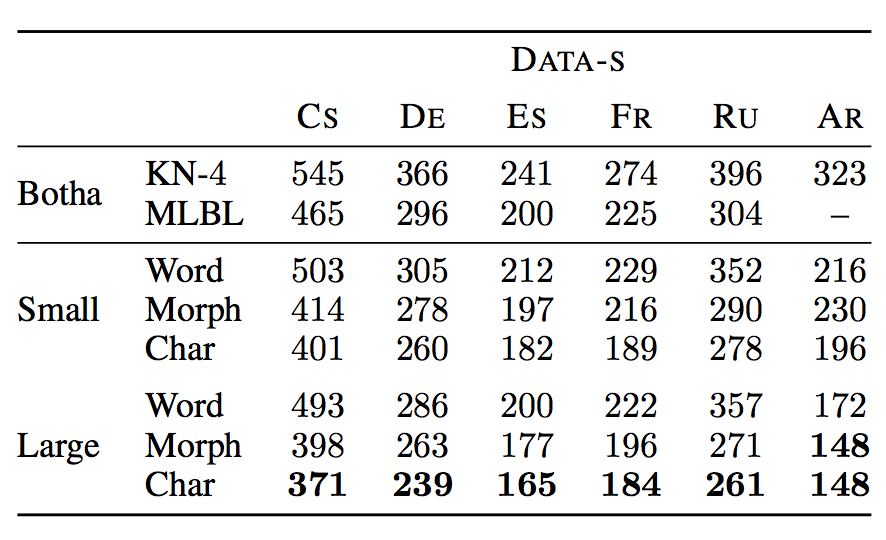
\includegraphics[width=0.6\textwidth]{./images/table4}
  \caption{对于DATA-S在测试集上的复杂度}
\end{figure}
\begin{figure}[h]
  \centering
  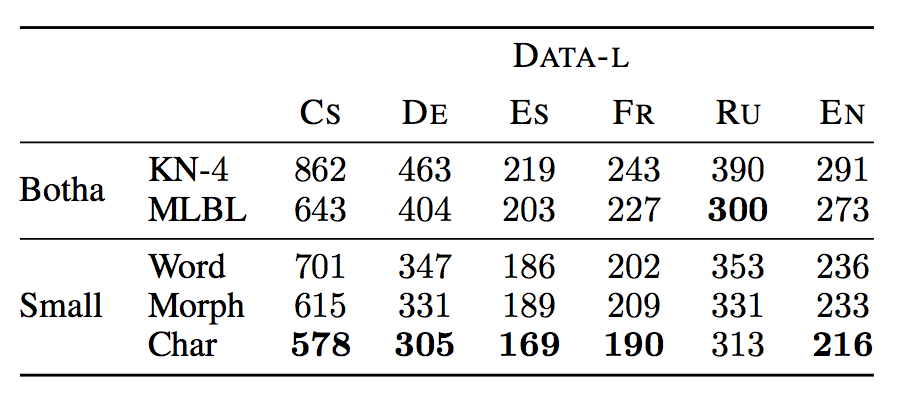
\includegraphics[width=0.6\textwidth]{./images/table5}
  \caption{对于DATA-L在测试集上的复杂度}
\end{figure}

\section{讨论}
\subsection{学习到的词表示}
\begin{figure}[h]
  \centering
  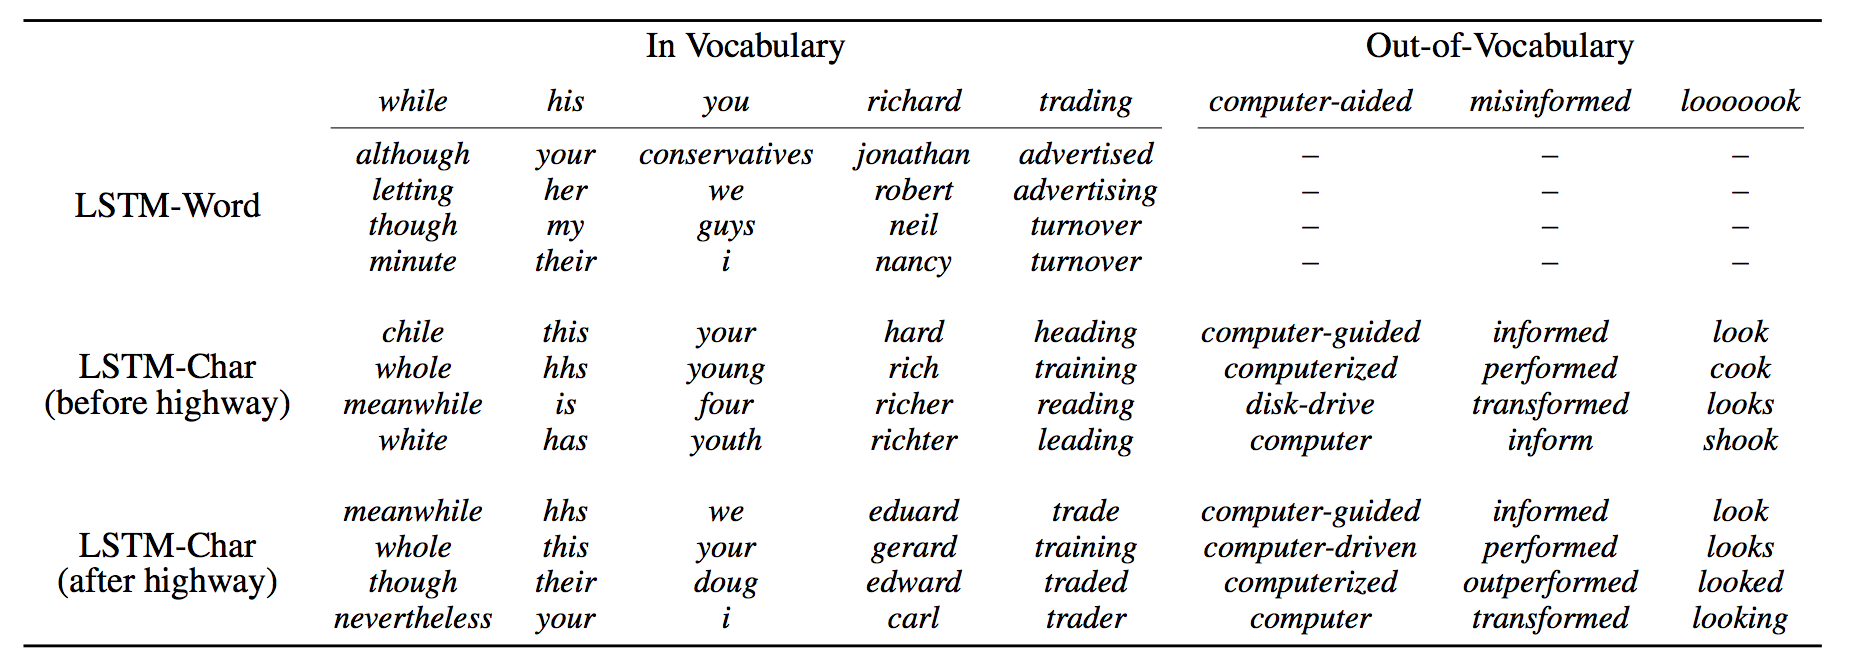
\includegraphics[width=0.95\textwidth]{./images/table6}
  \caption{最近邻词在字单位和词单位经过高速网络后的表达}
\end{figure}
我们研究了模型在PTB数据集上学习到的词的表示。表6显示了词单位和字单位模型学习到的近邻词表示。对于字单位模型,我们比较了使用高速网络前后的词表示。\\
在进入高速网络层之前,词表示看起来只依赖于表面形式,例如单词you的最近邻是your,young,four,youth。高速网络似乎能够编码和拼写无关的语义信息。
在经过高速网络之后,you的最近邻是we,we的拼写和you差很多。另一个例子是,while和though,他们看起来拼写很不一样,但是我们的模型能够把他们放置到临近的地方。
我们的模型也犯了很多明显的错误(比如his和hhs),尽管可能是由于数据集太小造成的,还是揭示了我们模型的一些局限。\\
\begin{figure}[h]
  \centering
  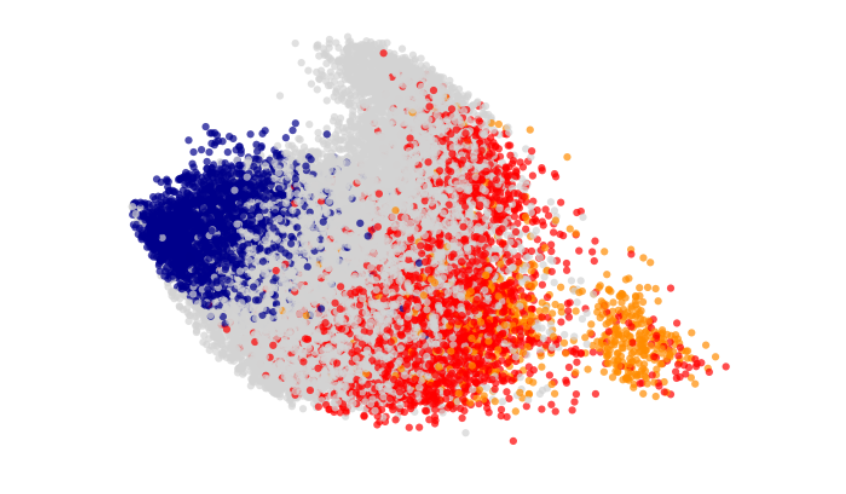
\includegraphics[width=0.6\textwidth]{./images/figure2}
  \caption{字的n元语法的点图}
\end{figure}
\subsection{学习到的字n元语法表示}
正如前面讨论到的,CharrCNN的每个筛选器对于识别特定字的n元语法是必要的。我们最初的期待是每个筛选器能够学习在不同的语素上激活,然后根据识别出的语素实现语义表达。
然而,通过研究筛选器选出的n元语法,我们发现它们并没有和合法的语素建立起联系。\\
为了能够建立起更好的关于字模型学了的什么的直觉,通过主成分分析,我们绘出了学习到的n元语法的表示。我们把每个字n元语法送入CharCNN,然后利用CharCNN的输出作为对应的字的固定维度的n元语法表示。
正如图表2显示的,我们的模型学习到了如何区分前缀(红)、后缀(蓝)和其他(灰)。我们也发现这个表达对于包含连字符的字n元语法表示特别敏感,我们的推测是因为连字符通常预示着这个词是演讲的一部分。\\

\subsection{高速网络层}
我们通过隔离分析定量的研究高速网络的作用。我们移除模型的一层高速网络层,发现模型的性能严重下降。因为性能的不同可能是由于模型大小减少所造成的,
我们也训练了一个将$\bf{y}^k$送入一个一层MLP,然后将它作为LSTM的输入。尽管可能是因为优化的问题,但是我们发现MLP效果也很差。\\
我们推测高速网络对于CNN来说是必要的。CNN已经在很多NLP任务中被证明是有效的方法。我们推测将高速网络结合进CNN中将会取得更好的结果。\\
我们也发现:(1)有一到两层高速网络是很重要的,但是进一步增加高速网络层数,并没有取得更优的结果。(2)在最大池化前设置更多的卷积网络并没有帮助。(3)高速网络对于使用词嵌入作为输入的模型并没有帮助。\\
\begin{figure}[h]
  \centering
  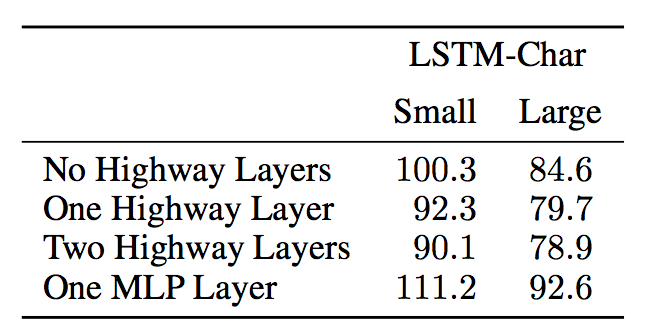
\includegraphics[width=0.6\textwidth]{./images/table7}
  \caption{小模型和大模型在使用/不使用高速网络的复杂度对比}
\end{figure}
\subsection{词汇量大小的影响}
我们接着学习了词汇集的大小对于不同模型结果的影响。我们使用DATA-L中的德语(DE)数据集,实用不同的词汇集大小,计算从词单位和字单位复杂率减少的大小。为了控制词汇量的变化,我们选出最常用的$k$个词,把他们替换为<unk>。
因为在前面的实验中,字模型没有使用<unk>的表面形式,只是把它当成另外一个标签。尽管表8表明随着词汇量的增加,复杂度减少的没有那么明显,我们还是发现字模型在所有的场景下都还是优于词模型。\\
\begin{figure}[h]
  \centering
  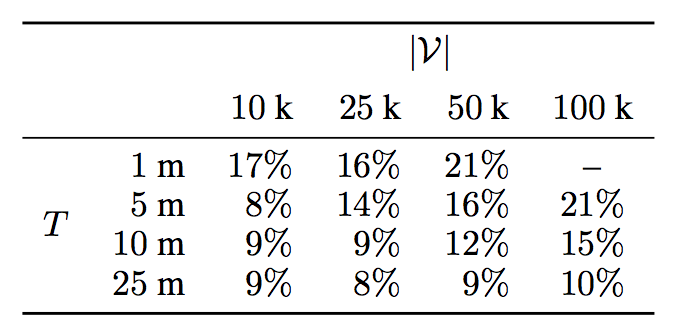
\includegraphics[width=0.6\textwidth]{./images/table8}
  \caption{不同的词汇量下,字模型比词模型在复杂度减少量}
\end{figure}
\subsection{进一步观察}
我们在进一步的的实验和观察中发现了下面的情况:
\begin{itemize}
\item 结合词嵌入和CharCNN的输出的词表示结果稍微糟糕一些。这个结果很让我们意外,因为有相关报道表明这样的结合在演讲标记和实体识别中有明显的改善。尽管我们的实验结果可能是 由于我们的实验设置的不够合理,
但是还是表明,对于一些任务,词嵌入式无用的,字输入就已经足够了
\item 尽管我们的模型需要卷积操作,所以相对于只是进行简单词查找的词模型慢一些,但是我们还是发现这种速度的区别可以通过GPU实现的优化来控制的。比如,在PTB数据集上,大的字单位模型训练速度为1500标签每秒,相对应的,
词模型训练速度为3000标签每秒。为了评分,因为CharCNN的输出可以被预先训练出来,所以我们的模型可以和词模型有相同的运行时间。然而,这样会增加模型的大小,所以这是一个在运行时速度和内存之间的取舍问题。
\end{itemize}
\section{总结}
我们引入了只使用字单位输入的神经语言模型。预测还是在词单位进行的,尽管模型有更少的参数,我们的模型表现超出使用词单位和使用语速单位的模型的基准线。
我们的模型对于词嵌入作为输入在神经语言建模中的必要性。\\
对于从字模型中获取到的词的表示进行分析之后揭示了这个模型能够只从字编码丰富的语义信息和拼写信息。使用CharCNN和高速网络层对于表达学习还是有很大帮助的。\\
到目前为止,由于序列化处理词作为自然语言处理比较普世的方法,如果这篇论文的方法能够对其他任务有所帮助是很好的。\\
\section{致谢}
我们非常感谢Jan Botha,他为我们提供了预处理好的数据和模型的结果。

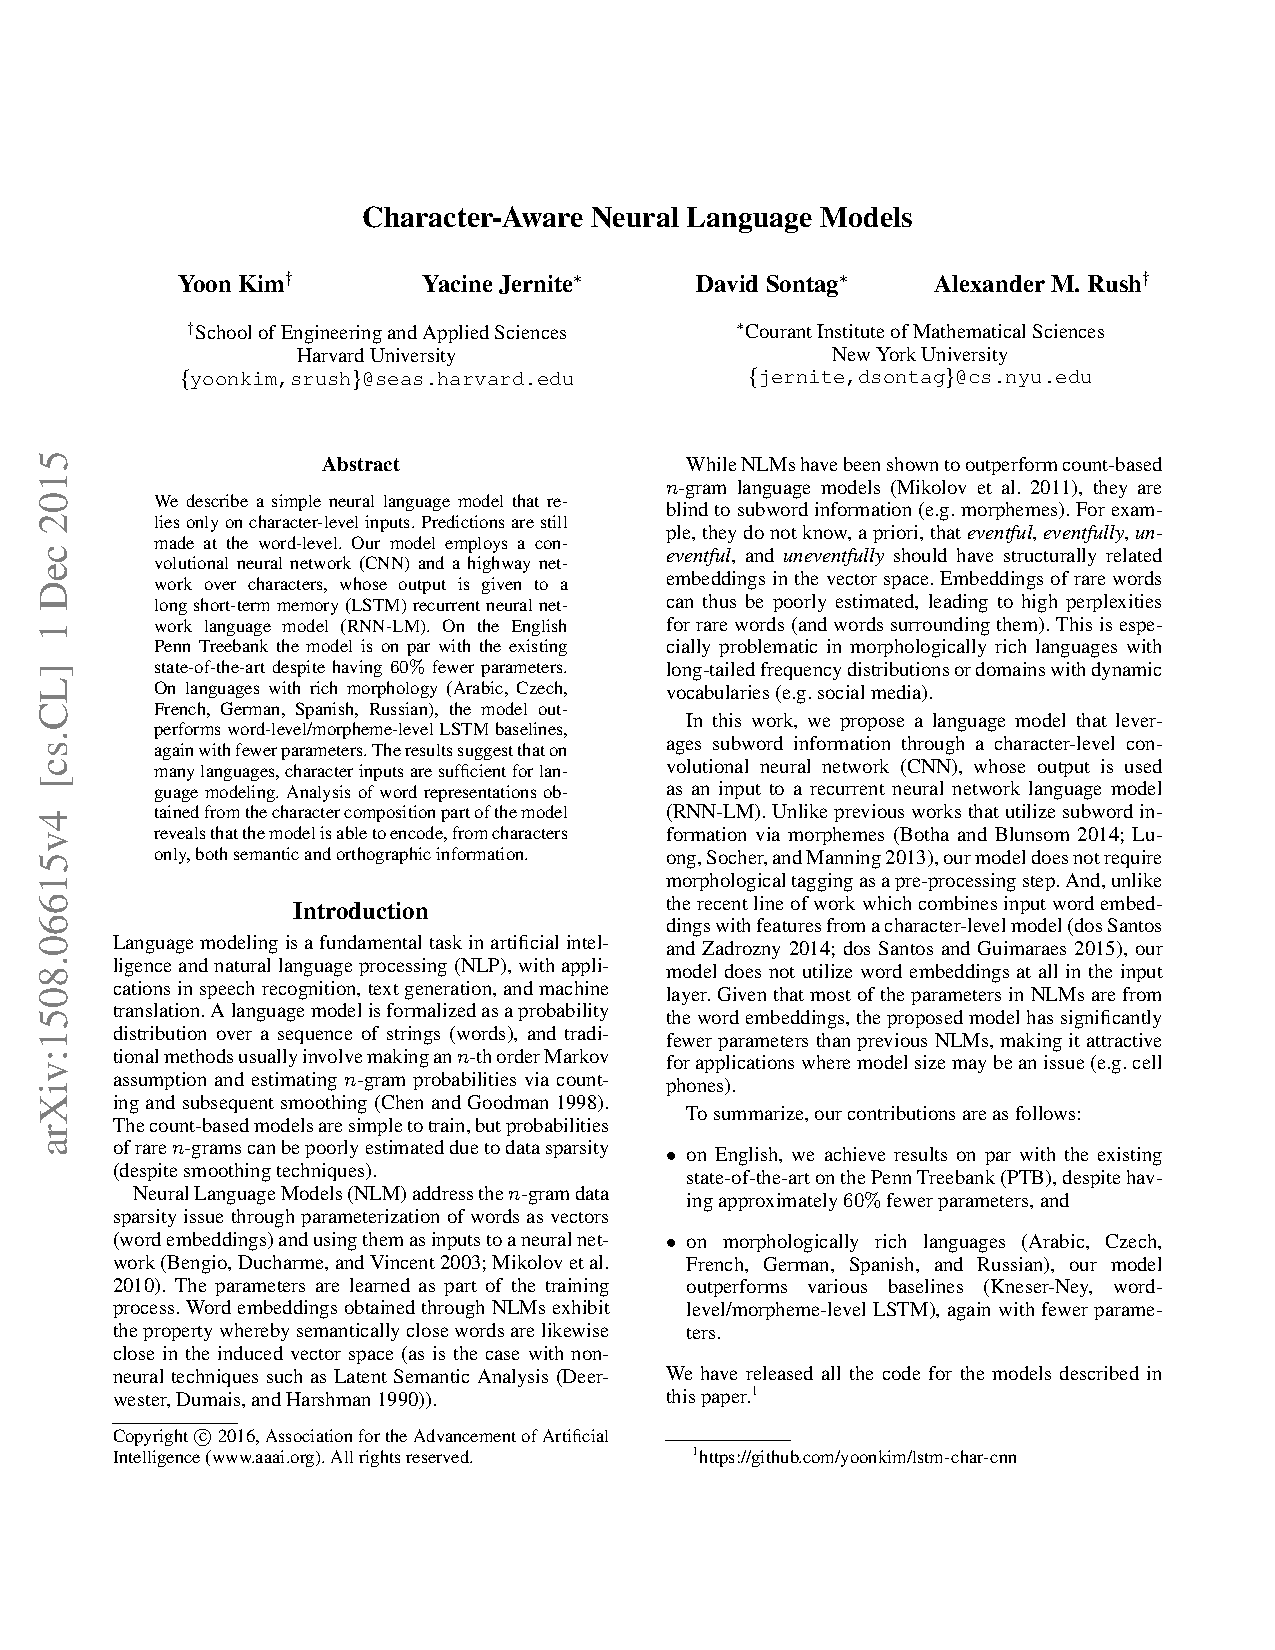
\includepdf[pages=-]{./data/translate-paper-english.pdf}
